\documentclass[10pt]{article}
\usepackage[margin=15mm]{geometry}
\usepackage{amsmath,amssymb,tikz,pgfplots}
\pgfplotsset{compat=1.18}
\definecolor{digitZero}{HTML}{246C91}
\definecolor{digitOne}{HTML}{BC632E}
\pagestyle{empty}
\begin{document}
\begin{center}
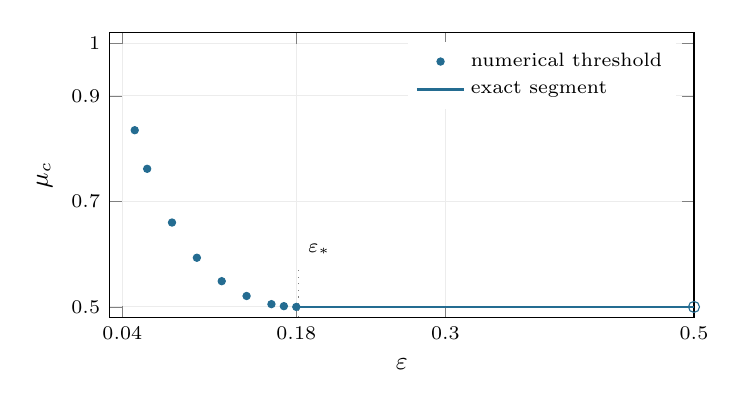
\begin{tikzpicture}
\begin{axis}[width=9cm,height=5.2cm,axis lines=box,
 tick label style={font=\scriptsize,/pgf/number format/fixed,/pgf/number format/precision=2,/pgf/number format/use period},
 label style={font=\small},title style={font=\small},scaled ticks=false,
 xmin=.03,xmax=.5,ymin=.48,ymax=1.02,xlabel={$\varepsilon$},ylabel={$\mu_c$},
 xtick={.04,.18,.3,.5},
 ytick={.5,.7,.9,1},grid=major,grid style={gray!15},
 legend style={font=\scriptsize,draw=none,fill=white},legend pos=north east,legend cell align=left]
\addplot[only marks,mark=*,mark size=1.3pt,digitZero] coordinates {(0.05,0.8349331969) (0.06,0.7617839431) (0.08,0.6599857676) (0.1,0.5932301704) (0.12,0.5488200012) (0.14,0.5207303402) (0.16,0.5052659873) (0.17,0.5014850523) (0.18,0.5000297083)};
\addlegendentry{numerical threshold}
% The unreliable epsilon=0.04 point is retained only in the numerical appendix.
\addplot[digitZero,thick] coordinates {(.181690113816,.5) (.5,.5)};
\addlegendentry{exact segment}
\addplot[gray,dotted,forget plot] coordinates {(.181690113816,.48) (.181690113816,.58)};
\node[font=\scriptsize,anchor=south west] at (axis cs:.181690113816,.58) {$\varepsilon_*$};
\addplot[only marks,mark=o,mark options={fill=white},digitZero,forget plot] coordinates {(.5,.5)};
\end{axis}
\end{tikzpicture}
\end{center}\end{document}
